\documentclass[12pt, a4paper]{article}

\usepackage[utf8]{inputenc}
\usepackage[french]{babel}
\usepackage{graphicx}
\usepackage{color}
\usepackage{hyperref}
\usepackage{amsthm}
\usepackage{tcolorbox}
\usepackage{enumitem}
\usepackage{amsfonts}
\usepackage[]{fullpage}
\usepackage{titlesec}
\usepackage{listings}

\graphicspath{{imgs/}}
\hypersetup{
    colorlinks,
    citecolor=black,
    filecolor=black,
    linkcolor=black,
    urlcolor=black
}

\title{Implantations efficaces de calculs sur les polynômes à une variable : FFT}
\author{a}
\date{7 Avril 2022}

\setcounter{secnumdepth}{4}

\begin{document}
\maketitle
\tableofcontents
\newpage

\section*{Introduction}
\addcontentsline{toc}{section}{Introduction}
Dans le cadre de l'UE LU2IN013, nous avons réalisé un projet sur l'optimisation de calculs sur les polynômes à une variable. Le but final de ce projet est la multiplication de deux polynômes sur $\mathbb{Z}/p\mathbb{Z}$ le plus efficacement possible.\\
Pour ce faire, nous nous intéressons à plusieurs type d'algorithmes pour la multiplication, en particulier : l'algorithme naïf, de Karatsuba et FFT.\\
Nous avons tout d'abord commencé avec Python mais nous avions besoin d'un langage bas niveau pour plus de rapidité d'où le fait qu'on a rapidement changé pour le C.

\section{Algorithme Naïf et de Karatsuba}
\subsection{Implémentations}

Pour commencer, nous avons réalisé un algorithme simple (l'algorithme naïf) de multiplication de deux polynômes $P$ et $Q$ de degrés $n$. Cette algorithme consiste à développer le produit comme on le ferait à la main, c'est-à-dire qu'on écrit : \\
\[R(X) = PQ(X) =
\displaystyle\sum_{i=0}^{n}\sum_{j=0}^{n} p_i q_j X^{i+j}\] \\
où $p_0,\dots,p_n\ et\ q_0,\dots,q_n$ sont les coefficients respectifs de $P$ et $Q$. Ici, à chaque tour de boucle, on rajoute aussi un modulo p pour que les coefficients restent sur $\mathbb{Z}/p\mathbb{Z}$.\\
De par sa simplicité, cette algorithme nous permet de vérifier les résultats de nos futurs algorithme plus performants mais plus complexe à implémenter.\\
Après cela, grâce aux différentes sources 
trouvés, nous avons implémenté l'algorithme de Karatsuba. (METTRE SOURCES)

\subsection{Comparaison - Naïf/Karatsuba}
L'algorithme naïf est en $O(n^2)$ et celui de Karatsuba en $O(n^{log_2(3)}) \approx O(n^{1.58})$ \\
(rajouter le nom des axes sur le graph. Ou faire un tableau ?) \\
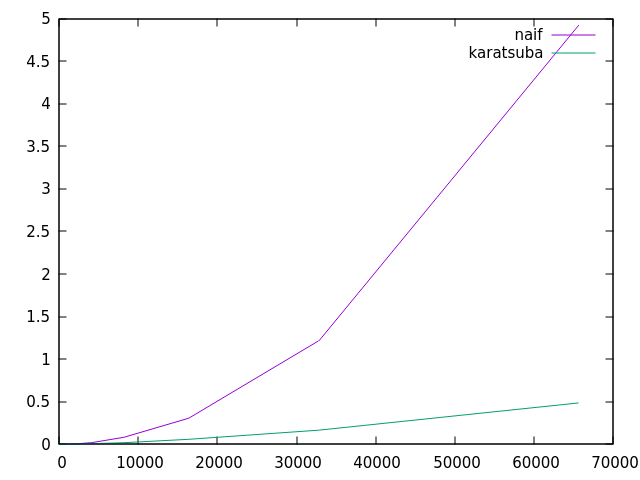
\includegraphics[scale=1]{naif_kara}\\

\section{Fast Fourier Transform (FFT)}

\newtheorem{Thm1}{Théorème}
\begin{Thm1}
Soient $a_1,\dots,a_n$ et $b_1,\dots,b_n$ des nombres réels (avec les $a_i$ deux à deux distincts). Aors il existe un unique polynôme P de degré n-1 tel que pour tout i dans $\{1,..., n\},\ P(a_i)\ =\ b_i$.
\end{Thm1}

La FFT se base sur ce théorème, en effet, l’idée est d’évaluer les polynômes $P$ et $Q$ en des points bien choisis, de faire le produits de ces évaluations et de retrouver l’unique polynôme $R=PQ$ à partir des valeurs du produit. Pour les points choisis, on prend les racines de l’unité car ?.
 
\begin{tcolorbox}[colback=cyan!5!white,
                  colframe=cyan!100!black,
                  title=\textbf{Algorithme FFT (METTRE SOURCES)}
                 ]
\textbf{Entrée.} $P$ et $Q$ deux polynômes, n un entier, et $\omega$ une racine principale n-ième de l’unité. \\
\textbf{Sortie.} $R = PQ$ \\
\textbf{Algorithme.}
\begin{enumerate}[itemsep=-2ex]
\item\textit{Précalcul}. Calculer les puissances $\omega^2,\dots,\omega^{n-1}$. \\
\item\textit{Évaluation}. Calculer les valeurs : \\ $Eval(P)=(P(\omega^0),\dots,P(\omega^{n-1}))$ ; $Eval(Q)=(Q(\omega^0),\dots,Q(\omega^{n-1}))$. \\
\item\textit{Produit point à point}. $Eval(R) = (PQ(\omega^0),\dots,PQ(\omega^{n-1}))$. \\
\item\textit{Interpolation}. On retrouve $R$ grâce à $Eval(R)$.
\end{enumerate}
\end{tcolorbox}
On voit que la complexité des étapes de précalcul et de produit point à point sont en $O(n)$, le problème est désormais de voir comment effectuer les étapes d'évaluation de d'interpolation rapidement.

\subsection{Évalution d'un polynôme (DFT)}

L'algorithme d'évaluation d'un polynôme est la deuxième étape de la FFT aussi appelé DFT (Discrete Fourier Transform), il se base sur le principe de diviser pour régner. 

\begin{tcolorbox}[colback=cyan!5!white,
                  colframe=cyan!100!black,
                  title=\textbf{Algorithme DFT (METTRE SOURCES)}
                 ]
\textbf{Entrée.} \\
\textbf{Sortie.} \\
\textbf{Algorithme.}
\end{tcolorbox}

Soient $n = 2^k\ et\ P(X) = p_n X_n +\dots+p_1 X + p_0$, on note $P_0$ et $P_1$ les polynômes de coefficients respectivement pair et impair de $P$, c'est-à-dire : \\
$P_0(X) = p_{n} X^{n/2} +\dots+ p_2 X + p_0\ et\ P_1(X) = p_{n-1} X^{n/2} +\dots+ p_3 X + p_1$. \\
On a alors que $P(X) = P_0(X^2)+X P_1(X^2)$. \\
La DFT se base sur cette propriété. En effet, on voit très vite qu'avec une telle décomposition, on peut faire un algorithme récursif où l'on divise le degré par deux à chaque fois.

\subsubsection{Utilisation des unsigned int (Uint)}

Comme nous travaillons sur $\mathbb{Z}/p\mathbb{Z}$, les coefficients des polynômes sont tous positifs. Cela nous permet de travailler avec des $unsigned\ int\ (Uint)$ et ainsi de travailler avec des entiers plus grands (jusqu’à $2^{32}-1$ au lieu de $2^{31}-1$ avec les $int$). Notre nombre premier valant initialement $p=2013265921$ $(2^{30} < p < 2^{31})$, les $Uint$ nous permettaient de pouvoir stocker la somme de deux entiers a et b entre $2^{30}$ et $p-1$, alors que ce n'était possible avec les $int$ car $a+b\geq2\times2^{30}=2^{31}$. \\
Malheureusement lors de l'implémentation de la vectorisation avec AVX2 dans notre code, nous avons vu qu'AVX2 ne permettait que de stocker des $int$, c'est pourquoi nous avons décidé de prendre un nombre premier plus petit, $p=754974721$ qui est entre $2^{29}$ et  $2^{30}$.

\subsubsection{Opérations modulo p}

Nous avons décidé de faire des fonctions d'addition, de soustraction et de multiplication de deux nombres avec modulo. Comme l'opération $\%$ prend environ 10 fois plus de temps que les opérations $+$ et $-$ en C, nous avons donc utiliser le fait que 
$ (a+b)\ \%\ p = 
\left\{\begin{array}{@{}l@{}}
a + b - p\ \ \ \ \ si\ a+b \geq p\\
a + b\ \ \ \ \ sinon
\end{array}\right.\,\ $ pour faire l'addition plus rapidement. \\
De même pour la soustraction on utilise que :
$ (a-b)\ \%\ p = 
\left\{\begin{array}{@{}l@{}}
p - (b - a)\ \ \ \ \ si\ b > a\\
a - b\ \ \ \ \ sinon
\end{array}\right.\,.$
Pour la multiplication nous avons quand même utilisé l'opération $\%$ tout en castant la multiplication en $long$ car la multiplication de deux coefficients peut facilement dépasser le nombre maximum des $Uint$. Il existe cependant des algorithmes plus efficaces pour faire le modulo dans la multiplication comme la réduction de Barrett qu'on va utiliser dans la troisième partie.

\subsubsection{Optimisation de la DFT}
Nous avons d'abord fait une première version fonctionnelle mais pas du tout optimisée de la DFT (voir la fonction $eval\_malloc()$) avec beaucoup de malloc inutiles. Par exemple, nous avons malloc, à chaque tour, les tableaux des polynômes $R_0$ et $R_1$ de l'algorithme. Nous avons alors décidé de faire un profilage de cette fonction et voici le résultat :
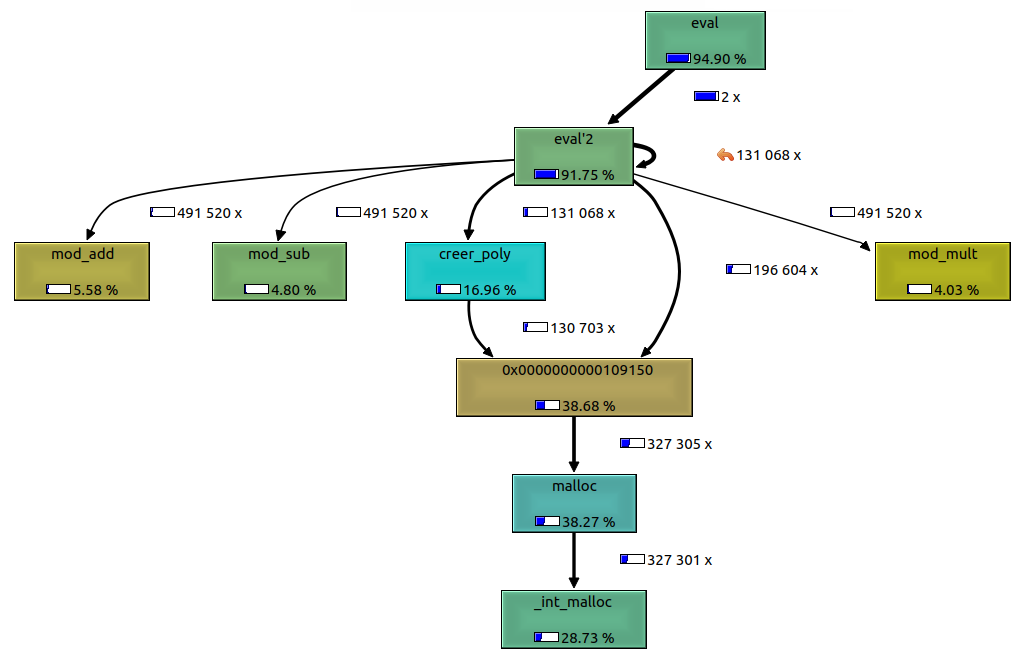
\includegraphics[scale=0.8]{profiler_eval_malloc}

On voit que les malloc représentent environ 40\% du temps d'exécution de la fonction ! \\
Pour optimiser cette fonction, notre priorité était alors de réduire le nombre de malloc. Nous avons d'abord remarqué qu'on pouvait enlever le malloc pour le tableau $racines\_bis$, en effet, ce tableau sert à stocker les valeurs des cases $0,2,\dots,n$ du tableau $racines$, donc on a pu se passer du tableau $racines\_bis$ en passant en paramètre un pas $pas\_rac$ qu'on multiplie par deux à chaque tour. \\
Pour le malloc des tableaux de $R_0$ et $R_1$ de tailles $n/2$, nous avons pu les enlever en remarquant qu'on pouvait stocker les coefficients de $R_0$ dans la première moitié du tableau de $P$ (de taille n) et ceux de $R_1$ dans la deuxième moitié. Ceci étant grâce au fait qu'on ai plus besoin de $P$ aux prochains tours de récursion.
Comme prévu la nouvelle fonction optimisée (fonction $eval()$) était environ 40\% plus rapide que la première version :

\begin{center}
\begin{tabular}{||c c c||}
\hline
Degré (+1) & $eval\_malloc()$ & $eval()$ \\
\hline\hline
$2^{16}$ & XX & XX \\
\hline
$2^{17}$ & XX & XX \\
\hline
$2^{18}$ & XX & XX \\
\hline
$2^{19}$ & XX & XX \\
\hline
$2^{20}$ & XX & XX \\
\hline
$2^{21}$ & XX & XX \\
\hline
$2^{22}$ & XX & XX \\
\hline
$2^{23}$ & XX & XX \\
\hline
$2^{24}$ & XX & XX \\
\hline
\end{tabular}
\end{center}

\subsection{Implémentation de la vectorisation dans la FFT avec AVX2}

Pour que notre FFT soit encore plus rapide, nous avons eu recours à la vectorisation avec AVX2. AVX2 nous permet de faire un certains nombres d'opération (addition, soustraction...) beaucoup plus rapidement qu'avec les opérateurs normaux de C. En effet, AVX2 permet de créer un type de variable ($\_\_m256i$) pouvant stocker 8 entiers de 32 bits (comme si c'était un tableau), ce qui correspond parfaitement avec ce quoi nous travaillons. AVX2 pouvant faire une opération élémentaire sur deux $\_\_m256i$ aussi vite qu'une opération élémentaire sur deux $int$ en C, on voit qu'on peut aller jusqu'à 8 fois plus vite avec AVX2. Voici un exemple de l'addition de deux $\_\_m256i$ en AVX2 : 

\begin{lstlisting}
__m256i a = _mm256_set_epi32(1, 2, 3, 4, 5, 6, 7, 8);
__m256i b = _mm256_set_epi32(1, 0, 1, 0, 1, 0, 1, 0);
__m256i x = _mm256_add_epi32(a, b);
// on a x == [2, 2, 4, 4, 6, 6, 8, 8]
\end{lstlisting}

\subsubsection{Opération modulo p avec AVX2}

Le problème avec AVX2 est qu'il n'y a pas d'opération modulo, de plus, comme on fait des opérations directement sur 8 entiers en même temps, il est difficile de faire le modulo comme dans la partie 2.1.2. Par exemple, pour l'addition supposons que $p = 7$, $\overrightarrow{a} = [6, 2, 0, 0, 0, 0, 0, 0]$, $\overrightarrow{b} = [4, 1, 0, 0, 0, 0, 0, 0]$ et $\overrightarrow{x} = \overrightarrow{a}+\overrightarrow{b}$, on a notamment $\overrightarrow{x}[0] = 10$ et $\overrightarrow{x}[1] = 3$, on devrait donc retirer $p$ pour faire le modulo sur $\overrightarrow{x}[0]$ mais alors on aurait $\overrightarrow{x}[1] = 3-7 = -4$, ce qui n'est pas bon.\\ 
Pour faire l'addition et la soustraction, il faut savoir qu'AVX2 nous permet de prendre les minimums "positif" sur chaque cases de deux $\_\_m256i$ (tous les nombres négatifs vont être converti en $Uint$), par exemple :\\ $min\_pos([1, 0],\  [0, -10]) = min([1, 0], \ [0,$ UINT\_MAX$-10] = [0, 0])$ et non $[0, -10]$. \\
Pour l'addition, après avoir eu $\overrightarrow{x} = \overrightarrow{a}+\overrightarrow{b}$, nous allons faire l'opération $min\_pos(\overrightarrow{x},\ \overrightarrow{x}-\overrightarrow{p})$ où \overrightarrow{p} est un $\_\_m256i$ ne contenant que des $p$. Ceci permet bien de faire le modulo car si $\overrightarrow{a}[i] + \overrightarrow{b}[i] \geq p$, alors $min\_pos()$ retourne $\overrightarrow{x}[i] - p$. Sinon on a $\overrightarrow{a}[i] + \overrightarrow{b}[i] < p$, donc $\overrightarrow{x}[i]-p < 0$, et après conversion en $Uint$, $\overrightarrow{x}[i]-p$ sera plus grand que \overrightarrow{x}[i] et donc l'opération retournera \overrightarrow{x}[i]. Ceci correspond bien aux cas de la partie 2.1.2. \\
C'est la même logique pour la soustraction $\overrightarrow{x} = \overrightarrow{a}-\overrightarrow{b}$, on prend $min\_pos(\overrightarrow{x},\ \overrightarrow{x}+\overrightarrow{p})$. \\
Pour la multiplication, nous avons utilisé l'algorithme de réduction de Barrett, nous nous sommes inspirés de cette source (METTRE SOURCE) qui montre comment faire cette algorithme avec vectorisation sur des entiers 16 bits.

\subsubsection{Tests de temps}
\begin{center}
\begin{tabular}{||c c c||}
\hline
Degré (+1) & Normal & AVX \\
\hline\hline
$2^{16}$ & XX & XX \\
\hline
$2^{17}$ & XX & XX \\
\hline
$2^{18}$ & XX & XX \\
\hline
$2^{19}$ & XX & XX \\
\hline
$2^{20}$ & XX & XX \\
\hline
$2^{21}$ & XX & XX \\
\hline
$2^{22}$ & XX & XX \\
\hline
$2^{23}$ & XX & XX \\
\hline
$2^{24}$ & XX & XX \\
\hline
\end{tabular}
\end{center}

\end{document}
